\documentclass{SBCbookchapter}
\usepackage[utf8]{inputenc}
\usepackage[T1]{fontenc}
\usepackage[english,brazilian]{babel}
\usepackage{hyperref}
\hypersetup{colorlinks=true,allcolors=black}
\usepackage{graphicx}
% \usepackage{natbib}
% \setlength{\bibsep}{0.0pt}

\usepackage{color}
\usepackage[colorinlistoftodos,prependcaption,textsize=tiny]{todonotes}
\newcommand{\rg}[1]{\todo[linecolor=blue,backgroundcolor=blue!25]{RG: #1}}

\title{Programando aplicações multimídia usando o\\GStreamer}
\author{Guilherme F.~Lima, Rodrigo C.\,M.~Santos e Roberto
G.\,~de~A.~Azevedo}

\begin{document}
\maketitle
\begin{abstract}
\begin{otherlanguage}{english}
This short course is an introduction to GStreamer, one of the main
free/open-source frameworks for multimedia processing.  We start presenting
GStreamer, its architecture and the dataflow programming model, and then adopt
a hands-on approach.  Starting with an example, a simple video player, we
introduce each concept of GStreamer's basic C~API and implement it over the
initial example incrementally, so that at the end of the course we get a
complete video player, with support for the usual playback operations
(start, stop, pause, seek, fast-forward, and rewind).  We also discuss
sample filters---elements that manipulate audio and video samples.  We
present the various filters nativelly available in GStreamer and show how one
can extend the framework by creating a plugin with a custom filter that rotates
video samples.  The only prerequisite for the short course is a basic knowledge
of the~C programming language.  At the end of the short course, we expect that
participants acquire a general view of GStreamer, and be able to create
simple applications and explore its more advanced features.
\end{otherlanguage}
\end{abstract}

\begin{resumo}
Este minicurso é uma introdução ao GStreamer, um dos principais
\emph{frameworks} de código livre/aberto para processamento de dados
multimídia.  Começamos apresentando o GStreamer, sua arquitetura e modelo de
programação baseado em \emph{dataflow}, e em seguida, adotamos uma abordagem
prática.  Partindo de um exemplo inicial, um \emph{player} de vídeo,
introduzimos cada conceito da API~C básica do GStreamer e o implementamos
sobre o exemplo, incrementando-o, de forma que ao final do minicurso obtemos
um \emph{player} de vídeo interativo completo, com suporte às
operações usuais de reprodução de vídeo (\emph{start}, \emph{stop},
\emph{seek}, \emph{fast-forward} e~\emph{rewind}).  Discutimos também filtros
de amostras---elementos que manipulam as amostras de áudio e vídeo.
Apresentamos os diversos filtros disponíveis no GStreamer nativamente e
mostramos como estender o \emph{framework} criando um \emph{plugin} com um
filtro simples que rotaciona amostras de vídeo.  O único pré-requisito para o
minicurso é um conhecimento básico da linguagem~C.  Ao final do minicurso,
esperamos que os participantes tenham uma visão geral do GStreamer, e estejam
aptos a criar aplicações simples e explorar os recursos mais avançados do
\emph{framework}.

\end{resumo}


%Justificativa de interesse e atração do público alvo
\section{Motivação}

O GStreamer~\cite{gstreamer} é um dos principais \emph{frameworks} de código
aberto para processamento de dados multimídia.  Além de robusto e flexível,
ele suporta diversos formatos de áudio e vídeo, sendo amplamente utilizado
na indústria e academia~\cite{gstreamer-apps}.  Neste minicurso,
apresentamos tanto a base conceitual do \emph{framework} quanto a parte
prática.  Na parte conceitual, discutimos o modelo de computação
\emph{dataflow} no qual o GStreamer se baseia, e que também é adotado por
outros sistemas multimídia, e.g., Pure Data~\cite{Puckette-M-S-2007},
CLAM~\cite{Amatriain-X-2008}, DirectShow~\cite{Chatterjee-A-1997}, etc.
Nesse modelo, uma aplicação multimídia estrutura-se como um grafo
(\emph{pipeline}) em que os nós são elementos processadores e as arestas
representam conexões entre elementos por onde fluem as amostras de áudio e
vídeo e dados de controle (cf.~Figura~\ref{fig:pipeline}).  O modelo de
\emph{dataflow} é particularmente interessante para multimídia porque
possibilita implementações naturalmente paralelas, modulares e
escaláveis~\cite{Yviquel-H-2014}.

\begin{figure}[ht!]
  \label{fig:pipeline}
  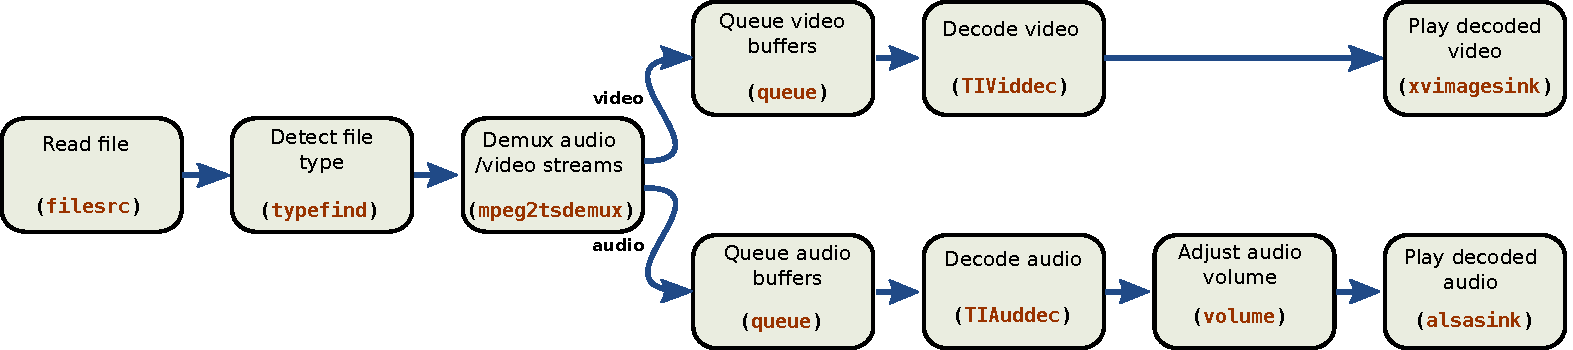
\includegraphics[width=\textwidth]{gstreamer_pipeline.pdf}
  \caption{Exemplo de um pipeline Gstreamer.}
\end{figure}

Na parte prática, apresentamos os principais conceitos da API~C básica do
GStreamer~1.8, sua versão estável mais atual, e ilustramos o uso dessa API a
partir da construção de um \emph{player} de vídeo.  Apesar de aqui estarmos
interessados apenas na reprodução (i.e., decodificação e apresentação) de
fluxos de mídia, essa mesma API pode ser utilizada para capturar fluxos de
áudio e vídeo, codificá-los e transmiti-los na rede.  O GStreamer suporta
nativamente uma grande variedade de componentes para tratar cada uma dessas
fases de processamento e, portanto, pode ser usado para construir diversos
tipos de aplicações multimídia, tais como editores de vídeo,
\emph{transcorders}, transmissores de fluxos de mídia, \emph{players} de
mídia, e \emph{players} de linguagens multimídia.  Dessa forma, acreditamos
que, não apenas programadores, mas boa parte do público do WebMedia pode
tirar algum proveito deste minicurso.


\section{Público-alvo}

O público-alvo deste minicurso são programadores, alunos de graduação e de
pós-graduação interessados em desenvolver aplicações multimídia.  Os
participantes devem possuir conhecimento básico da
linguagem~C~\cite{Kernighan-B-W-1988} e estarem familiarizados com algum
ambiente de desenvolvimento para essa linguagem.  Como o minicurso será
ministrado em GNU/Linux, é desejável que os participantes tenham
conhecimento básico desse tipo de ambiente.


\section{Sumário}
Este minicurso possui oito módulos.

\begin{enumerate}
\item\emph{Introdução ao GStreamer}.  Apresentação do \emph{framework}
  GStreamer (histórico, arquitetura básica, licença, quem usa, dependências,
  formatos e plataformas suportadas) e do seu modelo de programação
  (\emph{dataflow} multimídia).

\item\emph{Olá mundo: Tocando um vídeo}.  Apresentação do exemplo base: uma
  aplicação que toca um vídeo e termina.  O exemplo utiliza a API de
  alto-nível~\texttt{GstPlayer}, atualmente a forma mais simples de se
  reproduzir um áudio ou vídeo no GStreamer.

\item\emph{Conceitos básicos: Destrinchando o exemplo anterior}.  Discussão
  do que está por trás do código aparentemente simples do exemplo anterior.
  Começamos mostrando o \emph{pipeline} que a API~\texttt{GstPlayer} usa
  para reproduzir o vídeo e aproveitamos esse exemplo para introduzir os
  conceitos básicos do \emph{framework}, viz., \emph{element}, \emph{pad},
  \emph{caps}, \emph{clock}, \emph{buffer}, \emph{event}, \emph{message},
  \emph{bus}, \emph{bin} e \emph{pipeline}.  Após discutir cada conceito,
  voltamos à pratica e reimplementamos o exemplo anterior usando a API
  básica do GStreamer.\footnote{Apesar da API~\texttt{GstPlayer} simplificar
    a programação de reprodutores de mídia, ela é inflexível e limita os
    possíveis usos do framework.  Dessa forma, é importante que os
    participantes do minicurso conheçam a API básica do GStreamer e seu modo
    de operação.}  Ainda neste módulo, discutimos as
  ferramentas~\texttt{gst-inspect}, que consulta os elementos instalados no
  sistema, e ~\texttt{gst-launch}, que constrói um \emph{pipeline} na linha
  de comando.

\item\emph{Entrada e saída}.  Adição de suporte à entrada do usuário
  (teclado e mouse) ao exemplo anterior.  Concluímos o módulo mostrando como
  renderizar os quadros produzidos no exemplo numa janela específica do
  sistema.

\item\emph{Filtros}.  Apresentação dos principais filtros de aúdio e vídeo
  disponíveis no GStreamer e discussão de como podem ser integrados ao
  exemplo.  Nesse ponto, apresentamos o resultado da combinação do exemplo
  com diferentes filtros, e discutimos como os parâmetros dos filtros podem
  ser alterados em tempo de execução.

\item\emph{Pause, seek, fast-forward, rewind e step}.  Discussão do
  funcionamento e implementação das operações \emph{pause}, \emph{seek},
  \emph{fast-forward} e \emph{rewind} no exemplo.  Também analisamos os
  problemas envolvidos em cada uma dessas operações destacando as situações
  em que elas podem falhar.

\item\emph{Plugins}.  Apresentação da arquitetura de \emph{plugins} do
  GStreamer e implementação de um filtro de vídeo simples.  Além do código,
  mostramos como gerar um \emph{plugin} com esse filtro, instalá-lo, e
  utilizá-lo em conjunto com o exemplo original.

\item\emph{Conclusão}.  Discussão de tópicos avançados que não foram
  abordados nos módulos anteriores, e.g., alterações na topologia do
  \emph{pipeline} em tempo de execução, \emph{mixers}, sincronização de
  pipelines, captura e codificação de áudio e vídeo, transmissão na rede,
  \emph{bindings} em outras linguagens, etc.
\end{enumerate}


\section{Currículo dos autores}

\noindent\emph{Guilherme F.~Lima} é pesquisador associado do Laboratório
TeleMídia da PUC-Rio.  Seus interesses de pesquisa incluem linguagens de
programação e modelos para sincronismo multimídia.  Obteve o Doutorado em
Informática pela PUC-Rio em 2015.  Também possui Mestrado em Informática
(2011) e Bacharelado em Sistemas de Informação (2009), ambos pela PUC-Rio.

\noindent\emph{Rodrigo C.\,M.~Santos} é doutorando em Informática na
PUC-Rio.  Mestre em Ciência da Computação pela Universidade Federal do
Maranhão (2013).  Atualmente é pesquisador do laboratório TeleMídia/PUC-Rio
e colaborador do laboratório LAWS/UFMA, atuando principalmente na área de
sistemas multimídia.

\noindent\emph{Roberto G.\, de A.~Azevedo} é pesquisador associado do
Laboratório TeleMídia da PUC-Rio. Possui doutorado (2015) e mestrado (2010) em
Informática pela PUC-Rio e é Bacharel em Ciência da Computação pela
Universidade Federal do Maranhão (2008). Seus interesses de pesquisa incluem:
representação e autoria de cenas multimídia interativas; e representação,
codificação, transmissão e renderização de vídeos 3D.


\section{Apresentador do minicurso}

Rodrigo C.\,M.~Santos.


\section{Recursos necessários}

Precisamos apenas de um projetor multimídia e de uma rede sem fio com
internet.  Os participantes, se quiserem, podem desenvolver os exemplos em
seus computadores pessoais.


\bibliographystyle{plain}
\bibliography{bib}
\end{document}
